\newpage
\section{Empirical Evaluation}
\label{section:evaluation}
Please showcase your empirical results in this section. Please clearly specify which sets of experiments of the original paper are considered in your report. Please also report the corresponding hyperparameters of each experiment.

\subsection{Training History}

\begin{figure}[h!]
    \center
    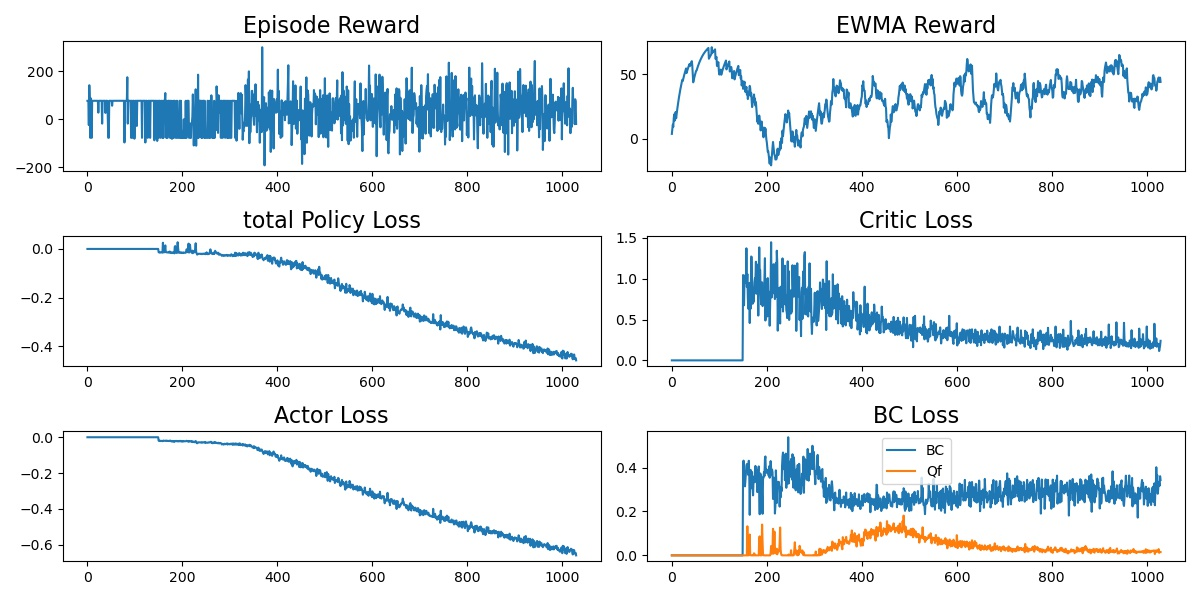
\includegraphics[width=15cm]
    {TrainCurve}
    \caption{The training curve}
    \label{fig: The training curve}
\end{figure}

This paper didn’t show any training history, so here shows our training results for the iRDPG agent. The total policy loss is the summation of actor loss and BC loss after Q-filter. For the first 150 episodes, we only conduct sampling without training.  So in the early training stage, the EWMA reward is relatively high because these are expert demonstrations. Then, from the BC Loss figure, the yellow curve is the BC loss after Q-filter. And we can see that the yellow curve decreases much, even though the original BC loss doesn’t decrease. It is evident that the iRDPG agent learns better policies than the expert as the training time goes by.


\subsection{Hyperparameters}

\begin{figure}[h!]
    \center
    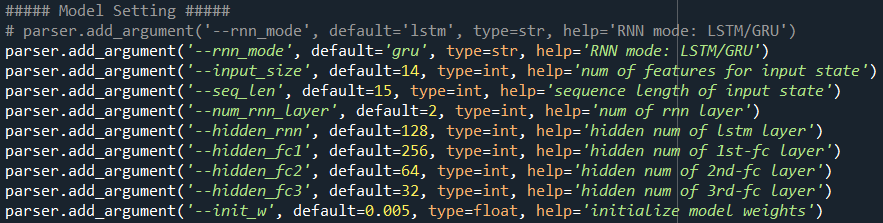
\includegraphics[width=15cm]
    {param_model}
    \caption{Parameters for agent model}
    \label{fig: param_model}
\end{figure}

Figure 6 presents the agent model setting. we can ether set the RNN layer as LSTM or GRU with two layers. The input size means input features which contain OHLC prices, buyline-selline of Dual Thrust, simple moving averages with previous 7 and 56 minites, RSI, KD, MACD, account profit and margin, etc. And the state sequence length is 15 minutes. In addition, both actor and critic has same three hidden layers but different input and output.

\begin{figure}[h!]
    \center
    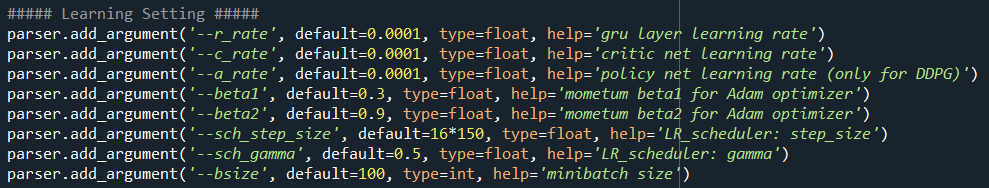
\includegraphics[width=15cm]
    {param_learning}
    \caption{Parameters for Adam optimizer and LR-scheduler}
    \label{fig: param_learning}
\end{figure}


\begin{figure}[h!]
    \center
    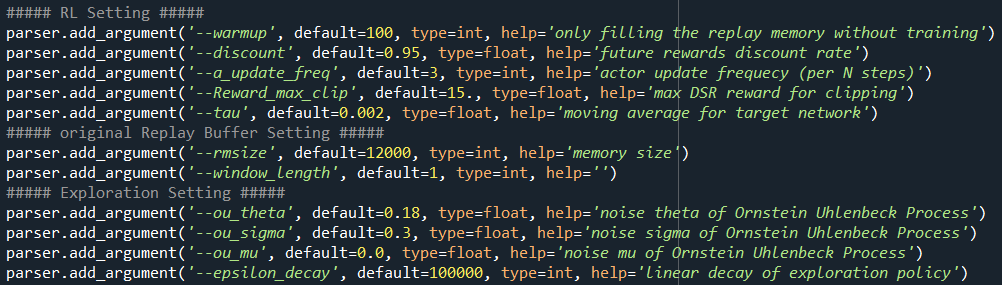
\includegraphics[width=15cm]
    {param_RL}
    \caption{Parameters for RL-algorithm, and random-process}
    \label{fig: param_RL}
\end{figure}

In figure 8, we set the warmup to be 100 episodes. Discount rate is 0.95. The soft replace rate is 0.002. Note, we update the actor every three step after updating the critic. Besides, the exploration is based on the Ornstein Uhlenbeck Process. 

\begin{figure}[h!]
    \center
    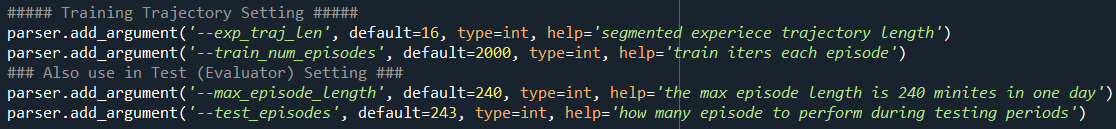
\includegraphics[width=15cm]
    {param_traj}
    \caption{Parameters for training trajectory}
    \label{fig: param_traj}
\end{figure}

In figure 9, the maximum steps of each episode is 240 since there are 240 trading minutes each day. And we segment every 16 steps to form an experience for train the recurrent DPG network. In addition, there are 243 trading days in the testing period.

\begin{figure}[h!]
    \center
    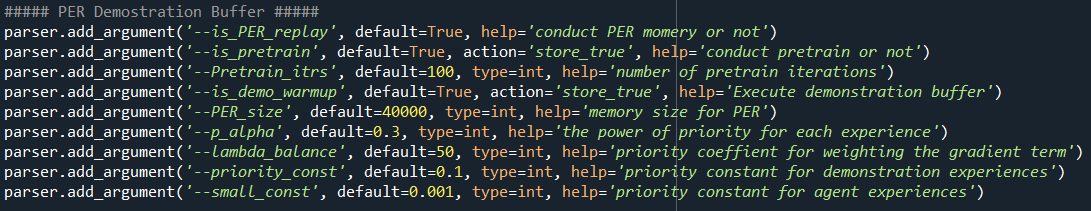
\includegraphics[width=15cm]
    {param_PER}
    \caption{Parameters for demonstration buffer and PER}
    \label{fig: param_PER}
\end{figure}

\begin{figure}[h!]
    \center
    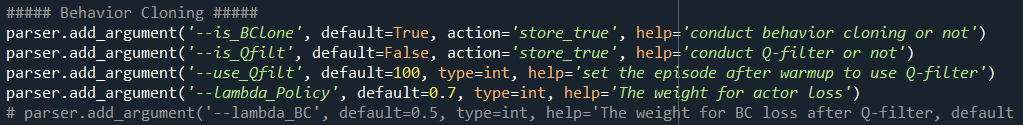
\includegraphics[width=15cm]
    {param_BC}
    \caption{Parameters for behavior cloning}
    \label{fig: param_BC}
\end{figure}


\begin{figure}[h!]
    \center
    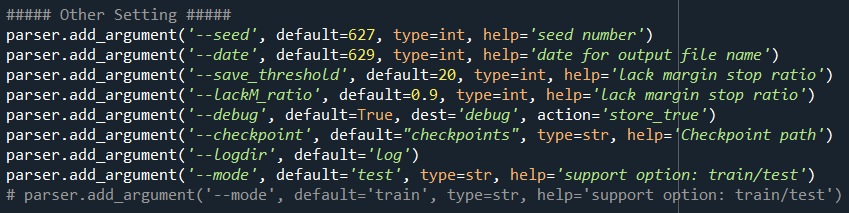
\includegraphics[width=15cm]
    {param_other}
    \caption{Parameters for other settings}
    \label{fig: param_other}
\end{figure}


\subsection{Ablation Experiments}

\begin{figure}[h!]
    \center
    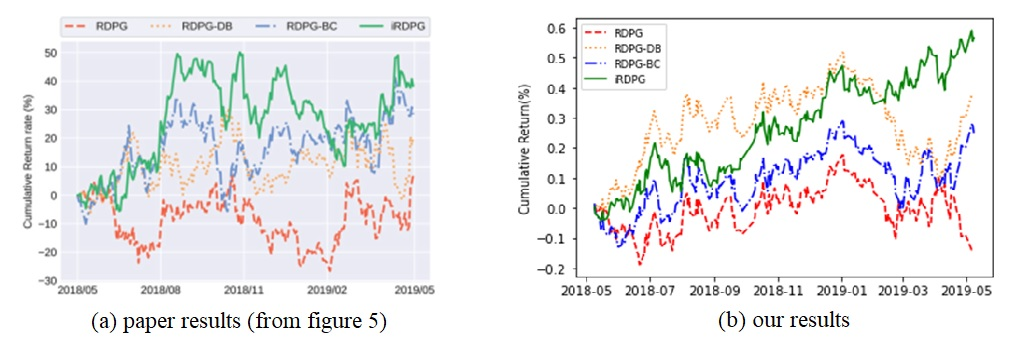
\includegraphics[width=15cm]
    {ablation}
    \caption{Cumulative return rates of ablation methods}
    \label{fig: ablation}
\end{figure}


This figure shows the comparison of ablation experiments. The LHS are the paper results (from Figure 5), and the RHS are our results. Both figures are the trading simulations by applying the trained agent to the one year test data (IF stock index futures from 2018/5/9 to 2019/5/8). And the four settings are RDPG, RDPG plus demonstration buffer (RDPG-DB), RDPG plus behavior cloning (BC), and the comprehensive iRDPG. Obviously, we can see that both results have similar trend, that is the iRDPG got the best trading performance. Also, we can find that if we train the RDPG without imitation technique, the RDPG trading performances are both not stable as shown by these two red curve.


\begin{figure}[h!]
    \center
    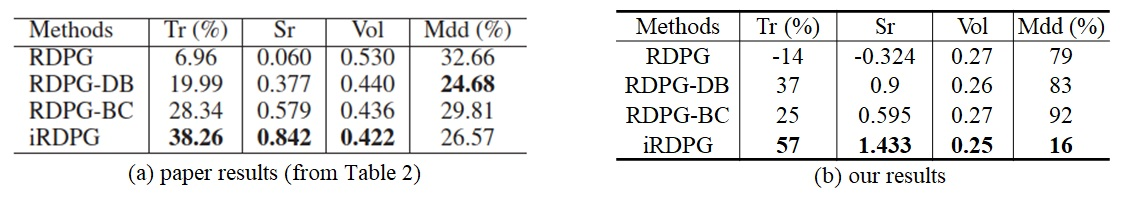
\includegraphics[width=13cm]
    {ablationTable}
    \caption{Ablation experiments of IF}
    \label{fig: ablationTable}
\end{figure}

The above two tables are the comparison of ablation trading performances on the following most widely used criteria. The LHS are the paper results (from Table 2), and the RHS are our results. Both tables are the trading performances by applying the trained agent to the one year test data (IF stock index futures from 2018/5/9 to 2019/5/8). Again, we can find that the iRDPG got the best performance. 

\begin{itemize}
    \item  Total return rate $\textbf{Tr}:=\frac{P_{end}-P_{start}}{P_{start}}$ ($P$ is the total value of the position and cash).
    \item Sharpe ratio $\textbf{Sr}:=\frac{\EX(\textbf{r})}{\sigma[\textbf{r}]}$ considers benefits and risks synthetically and reflects the excess return over unit systematic risk.
    \item  Volatility $\textbf{Vol}:=\sigma[\textbf{r}]$ (r denotes the historical sequence of return rate.) measures the uncertainty of return rate and reflects the risk level of strategies.
    \item  Maxium Drawdown $\textbf{Mdd}:=max\frac{(P_{i}-P_{j})}{(P_{i})},j>i$ measures the largest decline in history and shows the worst possible scenario.
\end{itemize}


\subsection{Generalization Ability}

\begin{figure}[h!]
    \center
    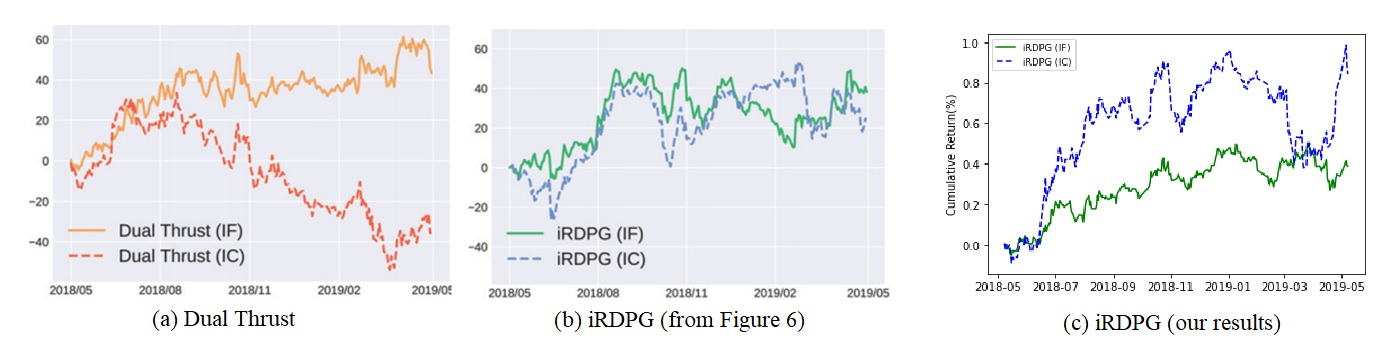
\includegraphics[width=15cm]
    {generalizability}
    \caption{Generalizability of iRDPG on IF and IC}
    \label{fig: generalizability}
\end{figure}

These figures present the generalizability of iRDPG agent. Figure(15-a) shows that if we apply the best parameter of Dual Thrust Strategy from IF to IC, it will fail as shown by the red curve. However, such failure will not happen by using the iRDPG agent. The iRDPG agent is trained in the IF training set and is tested in the IF and IC test set respectively. Figure(15-b) is the results from the paper Figure6, and Figure (15-c) is our implementation results. It is obvious that the agent got nice trading performance on both IF data and IC data. And such a trend in our results is consistent with the paper results. (Note: The reason why we can not successfully derive these results before the oral presentation on 6/23 is that we had different normalization settings for agent state value on IF and IC.)
